\documentclass[12pt]{article}
\usepackage[utf8]{inputenc}
\usepackage{polski}
\usepackage[a4paper, left=2.0cm, right=2.0cm, top=2.0cm, bottom=2.0cm]{geometry}
\usepackage{graphicx}
\usepackage{multicol}
\usepackage{hyperref}


\title{PIISW, W-4, IO, 2021/2022, semestr letni\\Lista zadań nr 2: JavaScript}
\author{mgr inż. Maciej Małecki\\\small{maciej.malecki@pwr.edu.pl}}

\begin{document}
    \maketitle

    \section*{Zasady oddawania zadań}
        \begin{enumerate}
            \item Zadania z~tej listy mogą być oddawane \emph{wyłącznie} za pośrednictwem prywatnego repozytorium na portalu \texttt{github.com}.
            \item Przed zajęciami, na których oddawana będzie lista należy nadać prowadzącemu uprawnienia do odczytu dla w.w. repozytorium.
            \item Rozwiązanie każdego z~zadań musi znaleźć się w~katalogu o~nazwie \texttt{zad-x} gdzie \texttt{x} jest numerem zadania.
            \item Rozwiązanie każdego z~zadań musi mieć nazwę \texttt{index.html}.
            \item Zadania należy zrealizować w~oparciu o~standardowe API przeglądarki, w~szczególności zabronione jest korzystanie z~bibliotek typu JQuery.
            \item Każde rozwiązanie powinno działać po otwarciu w.w. pliku w~przeglądarce Chrome (chyba, że w~zadaniu zaznaczono inaczej).
        \end{enumerate}

    \section*{Oceny}
    \begin{tabular}{|l|c|c|c|c|c|c|}
        \hline
        Punkty: & $<9$ & $9-10$ & $11-12$ & $13-14$ & $15-16$ & $17-18$\\
        \hline
        Ocena:  & $2,0$ & $3,0$ & $3,5$ & $4,0$ & $4,5$ & $5,0$\\
        \hline
    \end{tabular}

    \section*{Zadania}
        \begin{enumerate}
        \item\label{exc:dom-model}
            (5 pkt) Obsługa zdarzeń modelu DOM.

            Utwórz dokument HTML z~osadzonymi stylami oraz z~osadzonym kodem JavaScript, który wyświetli dwa elementy: kontrolkę suwaka oraz koło.

            \begin{enumerate}
                \item Przyjmij zakres dopuszczalnych wartości suwaka jako $10 - 500$.
                \item Średnica koła powinna być zawsze równa wartości ustawionej na suwaku (w~pikselach).
                \item Średnica koła powinna zmieniać się dynamicznie podczas przesuwania suwaka.
                \item Wewnątrz koła, w~jego geometrycznym środku powinna być zawsze wyświetlana jego średnica.
            \end{enumerate}


            Przykład wyglądu strony dla dwóch wybranych pozycji suwaka przedstawiono na rysunku~\ref{fig:dom-model}.

            Podpowiedź: koło można wyświetlić korzystając z~odpowiednio ostylowanego elementu \texttt{div}.

            \item\label{exc:forms}
            (6 pkt) Formularze i~walidacja.

            W~celu realizacji tego zadania użyj biblioteki styli Bootstrap: \url{https://getbootstrap.com/}.
            Użyj pliku \texttt{bootstrap.min.css} zawartego w~dystrybucji i~zintegruj go z~plikiem \texttt{index.html} będącym rozwiązaniem tego zadania.

            Zrealizuj formularz pozwalający na wprowadzenie: nazwy, szerokości, wysokości i~głębokości paczek.
            Wszelkie wymiary podawane są w~centrymetrach.

            Po zatwierdzeniu, nazwa oraz wymiary a~także wyliczona objętość paczki powinna zostać dodana jako kolejny wiersz w~tabeli znajdującej się poniżej formularza.
            Ponadto, w~stopce tabeli powinna być wyliczona sumaryczna objętość wszystkich paczek.

            Wygląd aplikacji powinien być zbliżony do tego z~rysunku~\ref{fig:forms}.
            Użyj odpowiednich styli z~pakietu Bootstrap aby to osiągnąć.

            Spełnij poniższe wymagania:
            \begin{enumerate}
                \item Wszyskie pola formularza są obowiązkowe.
                \item Pole nazwa powinno być polem tekstowym o~maksymalnej długości 20 znaków, pola wymiarów powinny być polami numerycznymi akceptującymi wartości całkowite z~przedziału od 1 do 1000~cm.
                \item Naciśnięcie przycisku Confirm powinno przede wszystkim zainicjować walidację pól i~wyświetlić odpowiednie komunikaty o~błędach.
                \item Naciśnięcie przycisku Clear powinno wyczyścić zawartość formularza.
                \item Wyliczana wartość objętości powinna być zaprezentowana w~metrach sześciennych oraz zaokrąglona do dwóch miejsc po przecinku.
                \item Użyj elementów semantycznych takich jak \texttt{form}, \texttt{table}, \texttt{input}, \texttt{label} oraz typów wejść jak \texttt{number}, \texttt{submit} oraz \texttt{reset}.
            \end{enumerate}

            Wskazówka: pakiet Bootstrap posiada wsparcie dla walidacji (patrz rysunek~\ref{fig:forms-error}) - pod warunkiem wykorzystywania możliwości, jakie daje HTML5 w~tym zakresie.

            \item\label{exc:notepad}
            (7 pkt) Notatnik i~składowanie danych
            Napisz prostą aplikację notatnika (widoczną na rysunku~\ref{fig:notepad}).
            Aplikacja powinna posiadać następujące funkcje:
            \begin{enumerate}
                \item Tworzenie nowej notatki składającej się z~tytułu i~treści. Tytuł jest obowiązkowy. Po kliknięciu przycisku ``Save'' notatka powinna zostać dodana do listy po lewej stronie a~formularz powinien zostać wyczyszczony.
                \item Wybór i~edycja zapisanej notatki. Po kliknięciu na jedną z~notatek na liście, zawartość notatki powinna wyświetlić się w~formularzu. Możliwa jest edycja zarówno tytułu jak i~treści - po kliknięciu ``Save'' notatka powinna być zaktualizowana, pola formularza powinny zostać wyczyszczone, nowy tytuł notatki powinien zostać odzwierciedlony na liście notatek.
                \item Notatki powinny zapisywać się w~pamięci ``localStorage'' przeglądarki - po wciśnięciu CTRL-F5 i~przeładowaniu strony, notatki powinny wciąż być widoczne.
            \end{enumerate}

            Przy ocenie tego zadania będziemy zwracać uwagę na styl:
            \begin{itemize}
                \item Należy zadbać o~możliwie dobrą separację logiki aplikacji i~warstwy wizualnej.
                \item Użyj obiektowości języka JavaScript tam, gdzie jest to potrzebne i~uzasadnione.
                \item Odseparuj stan lokalny aplikacji (lista notatek) oraz mechanizm utrwalania (localStorage) - niech twoim jedynym modelem nie będzie wartość z~localStorage!
                \item Zwróć uwagę, że tytuł notatki nie musi być unikalny - zaproponuj sposób jednoznacznej identyfikacji notatki.
            \end{itemize}

            Zwróć uwagę na subtelną różnicę stanu aplikacji: aplikacja bezpośrednio po uruchomieniu prezentuje pusty formularz, który po zapisaniu zawsze skutkuje utworzeniem nowej notatki. Gdy jednak notatkę wybierzemy z~listy, zapis skutkuje aktualizacją już istniejącej notatki.
            Zwróć uwagę także, że po naciśnięciu przycisku ``Save'' stan formularza powinien być identyczny jak po uruchomieniu aplikacji - pola są wyczyszczone a~formularz jest w~trybie wprowadzania \emph{nowej} notatki.

            Nie wolno używać dodatkowych bibliotek takich jak jQuery, Angular, React, itp. Wolno natomiast użyć Bootstrapa do stylowania widoku aplikacji.

            \begin{figure}[p]
                \centering
                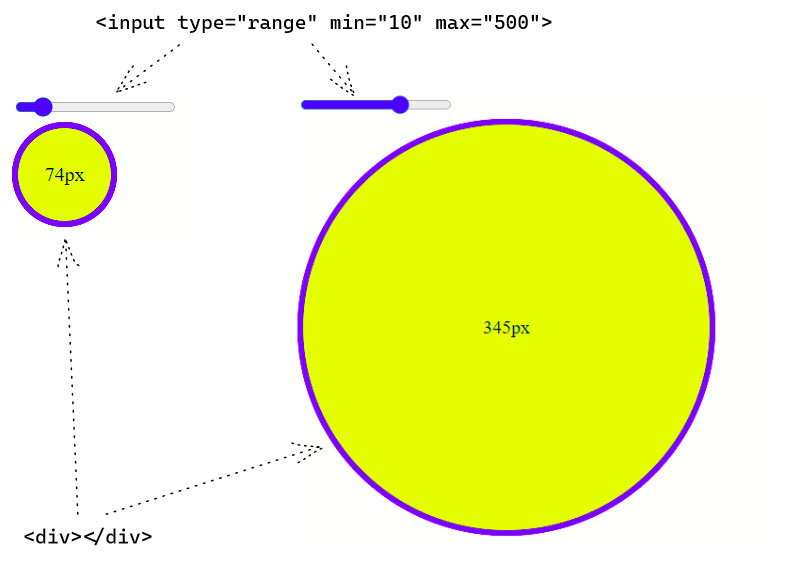
\includegraphics[width=0.8\textwidth]{lista-2-1}
                \caption{Dwie fazy działania kodu z~zadania~\ref{exc:dom-model}.}
                \label{fig:dom-model}
            \end{figure}

            \begin{figure}[p]
                \centering
                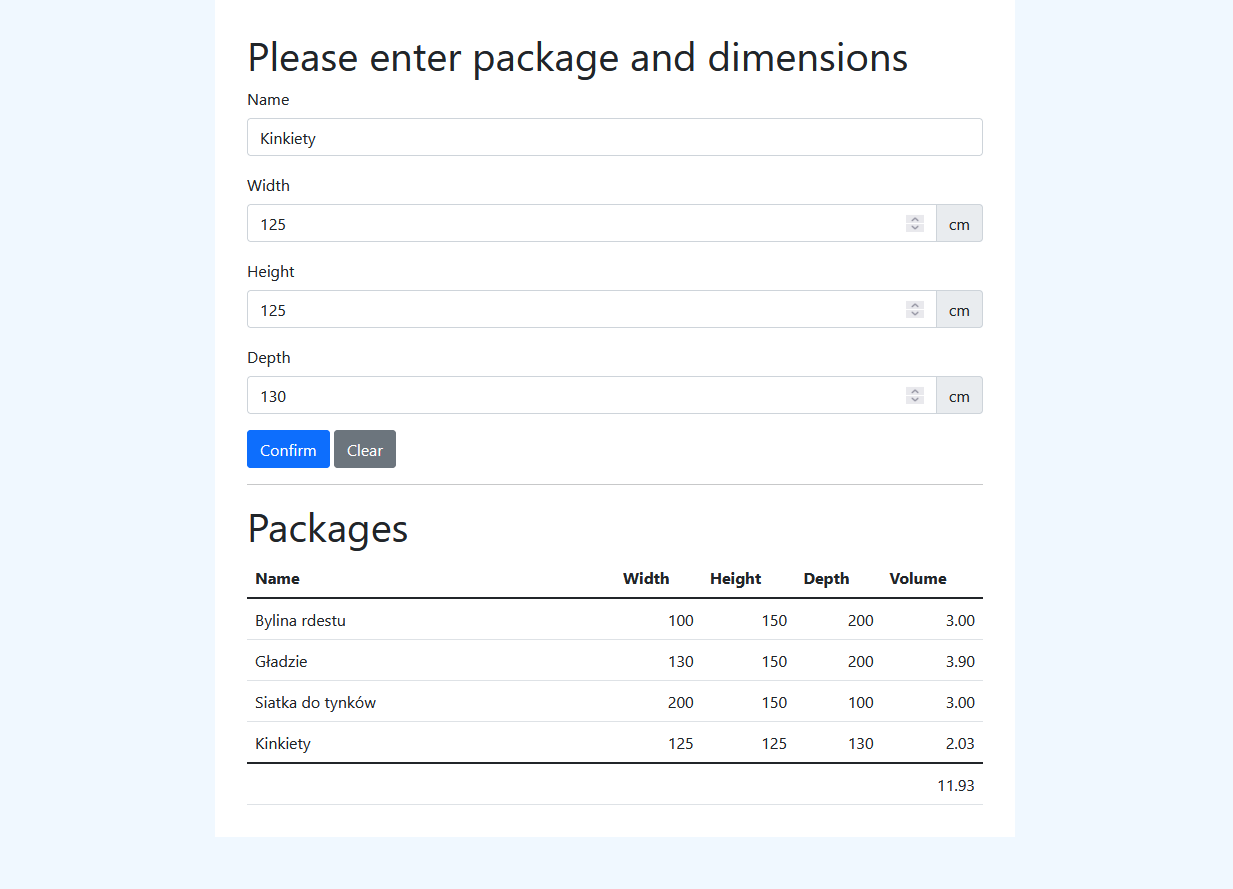
\includegraphics[width=0.9\textwidth]{lista-2-2}
                \caption{Przykład działania aplikacji z~zadania~\ref{exc:forms}.}
                \label{fig:forms}
            \end{figure}

            \begin{figure}[p]
                \centering
                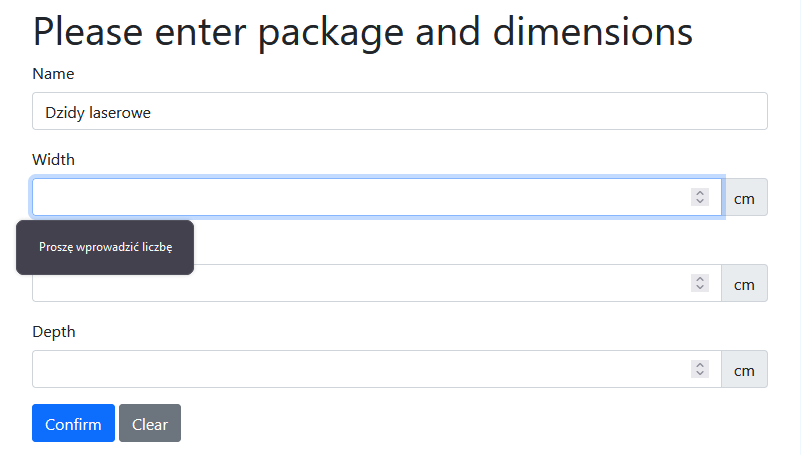
\includegraphics[width=0.75\textwidth]{lista-2-2-blad}
                \caption{Przykład działania walidacji formularza z~zadania~\ref{exc:forms}.}
                \label{fig:forms-error}
            \end{figure}

            \begin{figure}[p]
                \centering
                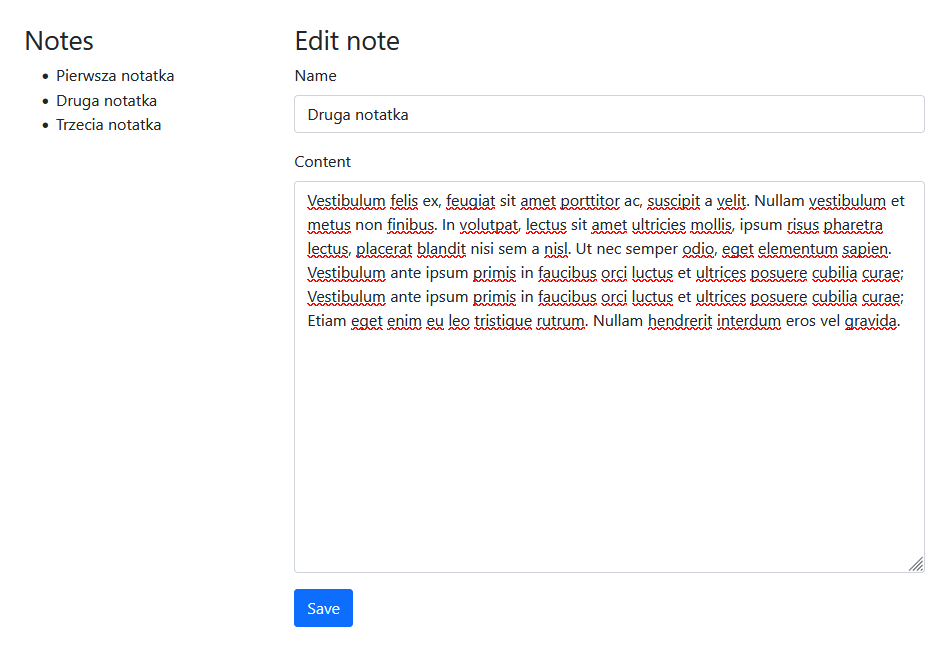
\includegraphics[width=0.75\textwidth]{lista-2-3}
                \caption{Aplikacja notatnika z~zadania~\ref{exc:notepad}.}
                \label{fig:notepad}
            \end{figure}

    \end{enumerate}
\end{document}

